\section{Introduction}
Les jeux d'enchères de type casino tels que le Poker, le Blackjack et bien d'autres sont considérés comme des jeux dit à information partielle. Évoluant de façon probabiliste, leur difficulté se caractérise par le fait qu'ils ne permettent pas aux joueurs de connaître à l'avance les gains exacts découlant de leurs actions. Dans cette optique, ainsi que dans le cadre de notre projet de programmation ayant pour but de réaliser un programme capable de jouer à ces jeux d'enchères, il nous est donc nécessaire de concevoir ce programme de manière à ce qu'il se base sur l'étude et le calcul des probabilités pour maximiser le gain final. Parmi les jeux d'enchères les plus populaires, nous avons décidé de focaliser notre projet sur le  Blackjack. En effet, nous considérons celui-ci comme étant un des plus abordables pour les joueurs. 

\section{Présentation du jeu}

Les sources utilisées pour la rédaction de cette partie ont été deux guides de Blackjack de sites spécialisés \cite{blackjack_regles_1} \cite{blackjack_regles_2}.

\subsection{Le Blackjack : un jeu de carte}

Le Blackjack est un jeu d'enchère qui utilise un jeu de carte classique de 52 cartes. Le paquet de carte comporte donc 4 couleurs (Coeur, Carreau, Pique, Trèfle) et pour chaque couleur il y a un As, des cartes numérotées de 2 à 10, un Valet, une Dame et un Roi.

\subsection{Les acteurs}

Les deux acteurs de ce jeu sont :
\begin{itemize}
    \item \textbf{La banque (le croupier)} qui distribue les cartes et joue "contre" les joueurs.
    \item \textbf{Les joueurs} qui misent et ceux-ci gagnent ou perdent en fonction de leurs cartes et des règles du jeu.
\end{itemize}

\subsection{Les règles du jeu en détail}

Tout d'abord, précisons que nous allons nous baser sur les règles officielles du Blackjack (appliquées dans les casinos aux États-Unis) et nous ne nous intéresserons pas aux différentes variantes qui peuvent exister comme le "Blackjack 6:5" ou encore le "Blackjack Royal Match".

\bigskip

Voici donc les règles officielles du Blackjack :

\begin{itemize}
    \item \textbf{Le nombre de joueur} \newline
    Une partie de Blackjack se joue avec un croupier et entre 1 et 7 joueurs.

    \item \textbf{Le but du jeu} \newline
    Chaque joueur a comme but d'atteindre 21 points avec ses cartes, sans le dépasser, ou battre le croupier.\\
    Un joueur bat le croupier lorsqu'il a plus de points que lui ou que le croupier dépasse 21 points.\\
    Un joueur perd lorsqu'il dépasse 21 points ou a moins de points que le croupier.\\
    Lorsqu'un joueur perd, il perd sa mise initiale, sinon, il la gagne avec un ratio dépendant de son score (explication ci-dessous).

    \item \textbf{Déroulement d'une partie}
    \begin{enumerate}
        \item Chaque joueur mise une somme d'argent.
        \item Le croupier distribue une carte face visible à chaque joueur ainsi qu'à lui-même. Il distribue ensuite une deuxième carte face visible à chaque joueur et se distribue une carte face cachée.
        \item Chaque joueur joue son tour de jeu.
        \item Le croupier joue son tour.
        \item Nous calculons les scores et les mises perdues/gagnées pour chaque joueur.
    \end{enumerate}
    
    
    \item \textbf{Un tour de joueur} \newline
    Un tour de joueur est composé de plusieurs actions. Son tour s'arrête lorsqu'il décide d'arrêter ou qu'il n'a plus le droit de faire des actions.\\
    Les différentes actions possibles sont :
    \begin{itemize}
        \item Demander une carte supplémentaire (piocher).
        \item S'arrêter de jouer (rester/se coucher/se retirer).
        \item Doubler sa mise et recevoir une carte. Après cette action, le tour du joueur est terminé.
        \item Abandonner. Le joueur perd alors la moitié de sa mise.
        \item \textbf{Cas spécial qui ne sera pas appliqué dans notre application : Le split} : Si le joueur se voit distribuer la carte en double (ex : 2 valets).
    \end{itemize}
    Un joueur n'a plus le droit de faire d'actions après s'être arrêté de jouer, avoir abandonné, doublé, ou perdu.
    
    \item \textbf{Un tour du croupier} \newline
    Le croupier tire des cartes tant qu'il a 16 points ou moins. Il s'arrête s'il a 17 points ou plus.

    \item \textbf{La valeur des cartes} 
    \begin{itemize}
        \item L'As : sa valeur peut être choisie, 1 ou 11.
        \item Les cartes numérotées (2, 3, 4, 5, 6, 7, 8, 9, 10) : valeur égale à la numérotation de la carte.
        \item Les figures (Valet, Dame, Roi) : valeur égale à 10.
    \end{itemize}

    \item \textbf{Décompte des scores} \newline
    Lorsque chaque joueur et le croupier ont fini leur tour, la partie est terminée et le décompte des scores est alors réalisé.
    Le score d'un joueur est la somme des valeurs de ses cartes.
    Si un joueur a 21 points avec seulement deux cartes, nous disons qu'il a un \textit{blackjack}.
    
    Voici ci-dessous un résumé précis et concis du décompte des scores, trouvable sur la page Wikipédia française du Blackjack : 

    \begin{itemize}\itshape
        \item \textbf{Les joueurs perdants} : Les joueurs ayant plus de 21 points perdent l'intégralité de leurs mises.

        \item \textbf{Les joueurs qui ont un blackjack :}
        Les joueurs récupéreront alors leurs mises. Si le croupier n'a pas de blackjack les joueurs gagnent en plus 1.5 fois leurs mises.
        
        \item \textbf{Les joueurs qui ont 21 points ou moins sans blackjack} 
        \begin{itemize}\itshape
            \item \textbf{Si le croupier a plus de 21 points} alors les joueurs récupèrent leurs mises de départ et gagnent en plus une fois leurs mises.
            \item \textbf{Si le croupier a 21 points ou moins (sans blackjack) :}
                \begin{itemize}
                \item Les joueurs ayant moins de points que le croupier perdent leurs mises.
                \item Les joueurs ayant autant de points que le croupier récupèrent leurs mises.
                \item Les joueurs ayant plus de points que le croupier récupèrent leurs mises et gagnent une fois leurs mises.
                \end{itemize}
        \end{itemize}
    \end{itemize}
\end{itemize}
\bigskip

\section{Analyse de l'existant}
Il existe de nombreuses Intelligences Artificielles capables de jouer à des jeux d'enchères qui se basent sur des informations partielles, principalement pour le Poker. Celles-ci peuvent être très intéressantes et sont capables de battre les meilleurs joueurs du monde dans certains cas comme les intelligences artificielles Deepstack \cite{deepstack} ou Libratus \cite{libratusBlog}.

Dans notre cas, nous nous intéressons aux IA pouvant jouer au Blackjack. Tout d’abord, il faut prendre en compte l'existence de multiples stratégies que nous pouvons bien sûr appliquer via un ordinateur, des plus basiques \cite{stratBasique} à des versions basées sur les probabilités \cite{blackjack_statistics} \cite{stratProba} afin d’obtenir par exemple les meilleurs gains possibles durant la partie. Précisons aussi qu’il a été décelé des stratégies improductives, que nous pouvons donc éviter dans le comportement de notre IA \cite{stratNull}.
Pour les algorithmes d’IA jouant au Blackjack, il y a peu de programmes accessibles (surtout comparé à ceux réservés au Poker). Néanmoins, il existe des projets proches de ce que nous cherchons comme un programme permettant de générer une base de données de mains de joueur possible (en fonction des paramètres de la partie) \cite{gitBJDataset}, ou encore des IA s’appuyant sur des méthodes de deep ou machine learning \cite{gitBJmachineLearning}. Ces dernières sont bien plus avancées que les précédentes, car en termes de temps de calcul et de réussite elles sont plus performantes  \cite{blogBJmachineLearning}. 

Néanmoins, la visibilité des algorithmes liés aux jeux d’argent (et particulièrement au Blackjack) reste très limitée, car il est question d’argent donc n’est pas accessible au public.
C’est pourquoi il est difficile pour nous de se baser sur un projet existant réellement convaincant et correspondant à ce que nous voulons, c’est-à-dire des intelligences artificielles qui jouent au Blackjack.

\section{Le logiciel à développer}

Le logiciel final se décompose en plusieurs sections distinctes : 
\begin{itemize}
    \item Un joueur du jeu. Un joueur donnera au moteur son action à chaque tour de jeu. Il peut être humain comme IA.
    \item Le moteur de jeu. Il sera responsable d'exécuter une partie de Blackjack entre plusieurs joueurs et de l'afficher.
    \item Le lanceur de moteur de jeu. Il sera responsable de créer le moteur et de le paramétrer correctement en fonction de ce que l'utilisateur du logiciel demandera.
\end{itemize}

Le moteur est un objet qui a un ensemble de joueur sur lesquels il peut demander l'action à jouer en fonction de l'état du jeu. Le moteur ne connaît pas (et n'a pas à connaître) comment le joueur va "réfléchir", c'est l'implémentation du joueur qui dictera sa réflexion.

Cela permet de pouvoir changer très facilement de type de joueur. Il peut ainsi y avoir un joueur qui "réfléchit" en lisant sur l'entrée standard, ou en calculant grâce à une IA.

De plus, le moteur et son affichage seront dissociés afin de pouvoir passer d'une interface textuelle à une interface graphique facilement.

\bigskip

Le lanceur de moteur de jeu permet de demander à l'utilisateur du logiciel comment il veut lancer une partie, c'est-à-dire combien de joueur, quels types de joueurs, etc. L'utilisateur rentrera ces paramètres avec des arguments de la ligne de commande, ou dans un fichier de paramètres. Voir les besoins pour plus d'informations (cf. \nameref{sec:launcher}).

\bigskip

Le logiciel fournira le lanceur de moteur de jeu, le moteur de jeu (cf. \nameref{sec:engine}), ainsi que deux implémentations de joueur par défaut, un joueur "humain" (cf. \nameref{sec:human}), et un joueur "IA" (cf. \nameref{sec:ia}).

\bigskip

\textbf{Résumé d'exécution du logiciel}

\begin{figure}[H]
    \centering
    
    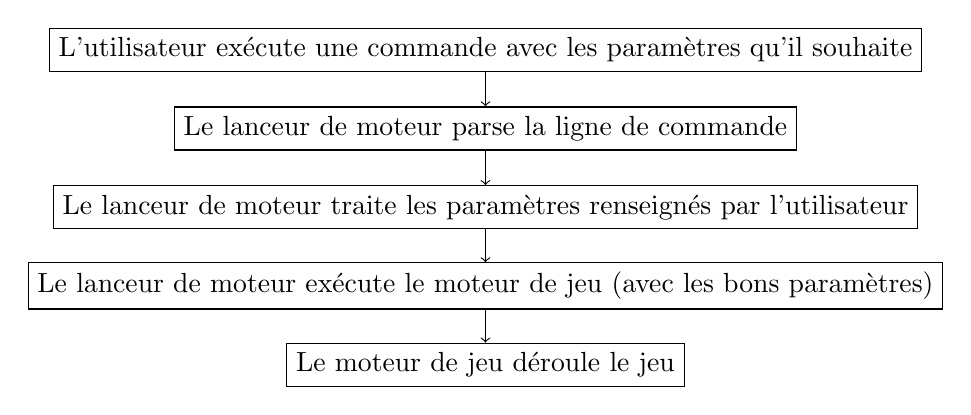
\begin{tikzpicture}
        \node[draw] (user) at (0,0) {L'utilisateur exécute une commande avec les paramètres qu'il souhaite};
        \node[draw] (parse) at (0,-1) {Le lanceur de moteur parse la ligne de commande};
        \node[draw] (param) at (0,-2) {Le lanceur de moteur traite les paramètres renseignés par l'utilisateur};
        \node[draw] (option) at (0,-3) {Le lanceur de moteur exécute le moteur de jeu (avec les bons paramètres)};
        \node[draw] (start) at (0,-4) {Le moteur de jeu déroule le jeu};
        
        \draw[->] (user) -- (parse);
        \draw[->] (parse) -- (param);
        \draw[->] (param) -- (option);
        \draw[->] (option) -- (start);
    \end{tikzpicture}
    
    \caption{Diagramme résumant les étapes d'exécution du logiciel}
    \label{fig:diag_exec}
\end{figure}

\clearpage

\textbf{Résumé du déroulement d'une partie (par le moteur de jeu)}

\begin{figure}[H]
    \centerline{
        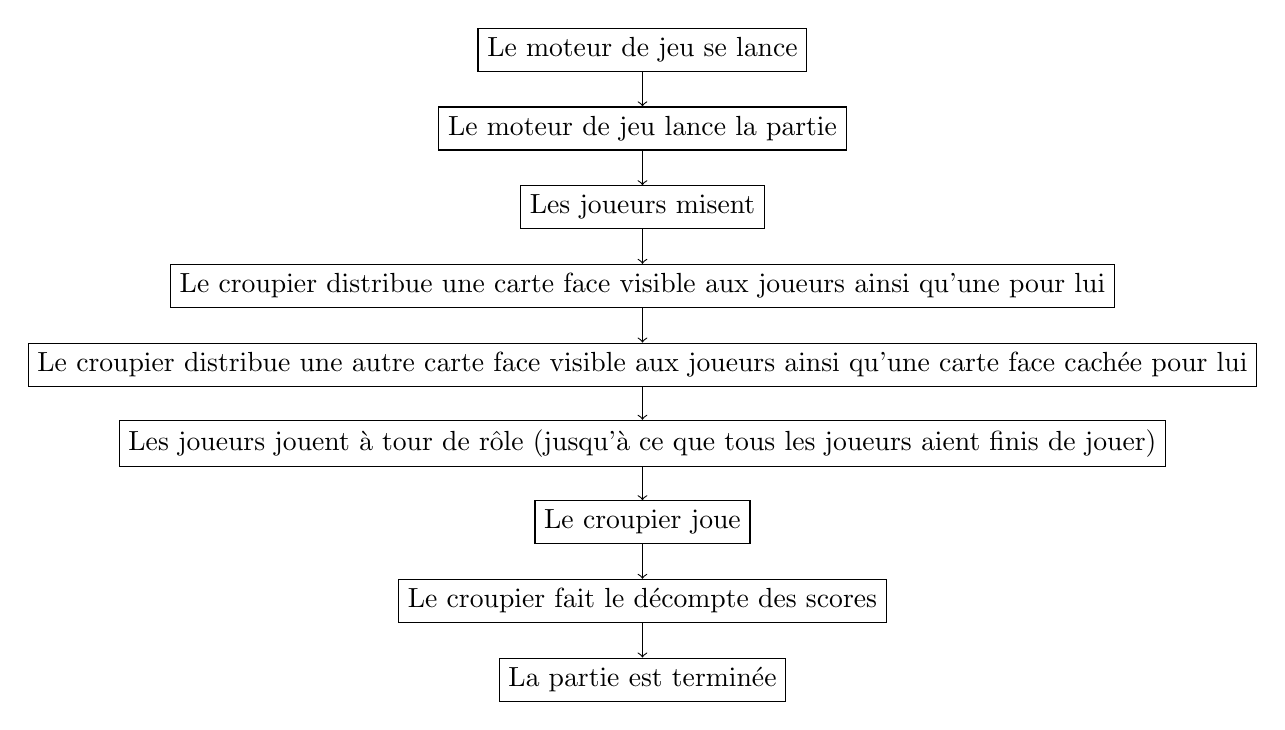
\begin{tikzpicture}[]
            \node[draw] (start1) at (0,0) {Le moteur de jeu se lance};
            \node[draw] (start2) at (0,-1) {Le moteur de jeu lance la partie};
            \node[draw] (bet) at (0,-2) {Les joueurs misent};
            \node[draw] (distrib1) at (0,-3) {Le croupier distribue une carte face visible aux joueurs ainsi qu'une pour lui};
            \node[draw] (distrib2) at (0,-4) {Le croupier distribue une autre carte face visible aux joueurs ainsi qu'une carte face cachée pour lui};
            \node[draw] (play1) at (0,-5) {Les joueurs jouent à tour de rôle (jusqu'à ce que tous les joueurs aient finis de jouer)};
            \node[draw] (play2) at (0,-6) {Le croupier joue};
            \node[draw] (score) at (0,-7) {Le croupier fait le décompte des scores};
            \node[draw] (end) at (0,-8) {La partie est terminée};
            
            \draw[->] (start1) -- (start2);
            \draw[->] (start2) -- (bet);
            \draw[->] (bet) -- (distrib1);
            \draw[->] (distrib1) -- (distrib2);
            \draw[->] (distrib2) -- (play1);
            \draw[->] (play1) -- (play2);
            \draw[->] (play2) -- (score);
            \draw[->] (score) -- (end);
        \end{tikzpicture}
    }

    \caption{Diagramme résumant les étapes d'un déroulement d'une partie avec x joueurs}
    \label{fig:diag_partie}
\end{figure}


\section{Outils utilisés}

Au cours de ce projet, nous avons eu l'occasion d'utiliser divers outils pour des parties précises du développement. 
Pour la réalisation des fichiers \LaTeX, nous avons utilisé l'application web Overleaf, celle-ci nous permettant de travailler à plusieurs facilement et simultanément. De plus, pour la gestion des tâches, nous avons porté notre dévolu sur l'interface web Trello, qui nous a permis de nous répartir aisément le travail tout au long de ce projet grâce à un tableau kanban. 
Pour le développement du code Python, nous avons employé PyCharm en tant qu'IDE et Visual Studio Code en tant qu'éditeur de texte. L'utilisation de ces logiciels a été individuelle et au gré des préférences de chacun. Enfin, nous nous sommes servis de Git et plus particulièrement de GitLab pour collaborer sur le code source et faire de la gestion de version.

\section{Fonctionnement du logiciel}

Dans l'état actuel, le lanceur et le moteur de jeu sont opérationnels et permettent d'effectuer plusieurs parties de 1 à 7 joueurs. Il est aussi possible d'utiliser différents types de joueurs IA, tous les détails pour les utiliser sont disponibles dans la notice d'utilisation du lanceur de moteur ou bien dans le README présent à la racine du projet.

\bigskip

\noindent Voyons ici un exemple simple de fonctionnement de l'application avec 2 parties réalisées par un joueur humain.

\subsection{Lancement du jeu}

Tout d'abord, l'utilisateur doit renseigner les différents arguments qu'il souhaite au lanceur de moteur afin que celui-ci puisse créer le moteur de jeu avec les bonnes valeurs.

\begin{figure}[H]
\begin{minted}
{md}
./run-launcher.sh -j humain -a 1000 -p 2 -d 2 -mn 10 -mx 500 -v

Paramètres de lancement:
  Joueurs : ['Human Player "humain 1":1000']
  Nombre de paquets : 2
  Mises : [10, 500]
  Nombre de parties : 2
  Verbeux : Oui
\end{minted}
\caption{Exemple d'utilisation du lanceur de moteur}
\label{fig:lancement_moteur}
\end{figure} 

Ensuite, la première partie commence et le moteur de jeu demande au joueur la mise qu'il souhaite faire. 

\begin{figure}[H]
\begin{minted}
{md}
humain 1
La mise minimale est : 10
La mise maximale est : 500
Vous avez : 1000
Veuillez entrer la mise que vous souhaitez mettre :
250
\end{minted}
\caption{Exemple de demande de mise pour un joueur humain}
\label{fig:exemple_demande_mise}
\end{figure} 

Lorsque toutes les mises sont renseignées, le moteur de jeu demande aux joueurs la ou les actions qu'ils souhaitent faire. 

\begin{figure}[H]
\begin{minted}
{md}
--------------- Table de jeu ---------------
Joueur "humain 1" :
  5♥ 9♠ (14)
  Mise: 250$
Croupier :
   7♦ ? (7)

humain 1
Veuillez entrer le code de l'action que vous souhaitez faire :
c - Tirer une carte
r - S'arrêter (rester)
d - Doubler sa mise (et recevoir une dernière carte)
a - Abandonner
d
\end{minted}
\caption{Exemple de demande d'action pour un joueur humain}
\label{fig:exemple_demande_action}
\end{figure} 

Une fois que tous les joueurs ont fini de jouer (qu'ils aient abandonné, doublé, brûlé ou qu'ils soient restés), le moteur de jeu fait jouer le croupier. Lorsque celui-ci a fini de jouer, le moteur de jeu calcule et affiche les résultats de la partie.

\begin{figure}[H]
\begin{minted}
{md}
Résultat pour "humain 1" :
  5♥ 9♠ 5♦ (19)
  humain 1 a gagné 500$
  humain 1 a 1500$

Croupier :
  7♦ 2♣ 4♣ 9♣ (22)
\end{minted}
\caption{Exemple d'affichage du résultat d'une partie}
\label{fig:exemple_affichage_resultat_partie}
\end{figure} 

Ensuite, s'il reste encore des parties à jouer et qu'un ou plusieurs joueurs peuvent encore jouer, le moteur de jeu lance la partie suivante.

\begin{figure}[H]
\begin{minted}
{md}
humain 1
La mise minimale est : 10
La mise maximale est : 500
Vous avez : 1500
Veuillez entrer la mise que vous souhaitez mettre :
400

--------------- Table de jeu ---------------
Joueur "humain 1" :
  10♦ K♠ (20)
  Mise: 400$
Croupier :
   9♦ ? (9)

humain 1
Veuillez entrer le code de l'action que vous souhaitez faire :
c - Tirer une carte
r - S'arrêter (rester)
d - Doubler sa mise (et recevoir une dernière carte)
a - Abandonner
r

Résultat pour "humain 1" :
  10♦ K♠ (20)
  humain 1 a gagné 400$
  humain 1 a 1900$

Croupier :
  9♦ 10♠ (19)
\end{minted}
\caption{Exemple complet d'une partie de Blackjack avec un joueur humain}
\label{fig:exemple_partie_complete}
\end{figure} 

Enfin lorsque toutes les parties ont été jouées, le moteur de jeu affiche l'argent de tous les joueurs.

\begin{figure}[H]
\begin{minted}
{md}
Résultat des parties :
  humain 1 a 1900$
\end{minted}
\caption{Exemple d'affichage du résultat final de plusieurs parties}
\label{fig:exemple_affichage_resultat_parties}
\end{figure} 